\documentclass[aspectratio=169]{beamer}

% ── Theme & Colors ────────────────────────────────────────────────────────────
\usetheme{AnnArbor}
\usecolortheme{default}

\definecolor{darkgreen}{RGB}{10, 75, 50}
\definecolor{midgreen}{RGB}{20, 120, 70}
\definecolor{accentgreen}{RGB}{0, 170, 90}
\definecolor{softgray}{RGB}{245, 248, 245}
\definecolor{alertred}{RGB}{180, 30, 40}
\definecolor{deepblue}{RGB}{20, 40, 100}

\setbeamercolor{palette primary}{bg=darkgreen, fg=white}
\setbeamercolor{palette secondary}{bg=midgreen, fg=white}
\setbeamercolor{palette tertiary}{bg=accentgreen!80!black, fg=white}
\setbeamercolor{palette quaternary}{bg=darkgreen, fg=white}
\setbeamercolor{structure}{fg=darkgreen}
\setbeamercolor{section in toc}{fg=darkgreen}
\setbeamercolor{block title}{bg=darkgreen, fg=white}
\setbeamercolor{block body}{bg=softgray, fg=black}
\setbeamercolor{block title alerted}{bg=alertred, fg=white}
\setbeamercolor{block body alerted}{bg=alertred!8, fg=black}
\setbeamercolor{block title example}{bg=deepblue, fg=white}
\setbeamercolor{block body example}{bg=deepblue!7, fg=black}
\setbeamercolor{frametitle}{bg=darkgreen, fg=white}
\setbeamercolor{title}{fg=white}
\setbeamercolor{subtitle}{fg=accentgreen!60!white}

% ── Packages ──────────────────────────────────────────────────────────────────
\usepackage{amsmath, amssymb}
\usepackage{mathtools}
\usepackage{tikz}
\usetikzlibrary{arrows.meta, positioning, shapes.geometric, calc, decorations.pathreplacing}
\usepackage{booktabs}
\usepackage{xcolor}
\usepackage{bm}

% ── Beamer Settings ───────────────────────────────────────────────────────────
\setbeamertemplate{navigation symbols}{}
\setbeamertemplate{itemize items}[circle]
\setbeamertemplate{enumerate items}[default]
\setbeamerfont{title}{size=\Large, series=\bfseries}
\setbeamerfont{frametitle}{size=\large, series=\bfseries}

\newcommand{\highlight}[1]{{\color{accentgreen!70!black}\textbf{#1}}}
\newcommand{\alerttext}[1]{{\color{alertred}\textbf{#1}}}
\newcommand{\JJ}{J_{\mathrm{VRFT}}}
\newcommand{\Jopt}{J}

% ── Title ─────────────────────────────────────────────────────────────────────
\title[Nonlinear VRFT]{Direct Nonlinear Control Design}
\subtitle{The Virtual Reference Feedback Tuning (VRFT) Approach}
\author[Campi \& Savaresi]{Marco C.~Campi \and Sergio M.~Savaresi}
\institute[]{Università di Brescia \quad \& \quad Politecnico di Milano}
\date{\textit{IEEE Transactions on Automatic Control}, Vol.~51, No.~1, January 2006}

% ══════════════════════════════════════════════════════════════════════════════
\begin{document}
% ══════════════════════════════════════════════════════════════════════════════

\begin{frame}[plain]
  \titlepage
\end{frame}

\begin{frame}{Outline}
  \tableofcontents
\end{frame}

% ══════════════════════════════════════════════════════════════════════════════
\section{Introduction \& Motivation}
% ══════════════════════════════════════════════════════════════════════════════

\begin{frame}{Why Data-Based Nonlinear Control Design?}
  \begin{columns}[T]
    \begin{column}{0.52\textwidth}
      \begin{alertblock}{Industrial Reality}
        \begin{itemize}
          \item Mathematical models of nonlinear plants are often \alerttext{unavailable}
          \item Deriving them is too costly and time-consuming
          \item Even when available, nonlinear models are often too complex for direct design
          \item Simulators can serve as data generators --- keeping the real plant undisturbed
        \end{itemize}
      \end{alertblock}
    \end{column}
    \begin{column}{0.45\textwidth}
      \begin{block}{Data-Based Design Paradigm}
        \centering
        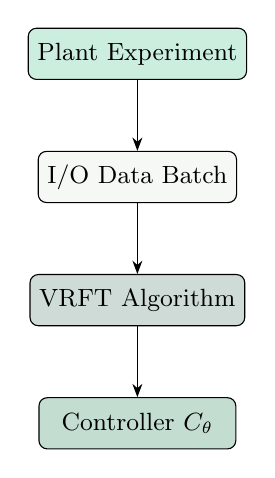
\begin{tikzpicture}[node distance=0.9cm,
            box/.style={draw, rectangle, rounded corners=3pt, minimum width=2.5cm, minimum height=0.65cm, font=\small, align=center},
            >=Stealth]
          \node[box, fill=accentgreen!20] (exp) {Plant Experiment};
          \node[box, fill=softgray, below=of exp] (data) {I/O Data Batch};
          \node[box, fill=darkgreen!20, below=of data] (alg) {VRFT Algorithm};
          \node[box, fill=midgreen!25, below=of alg] (ctrl) {Controller $C_\theta$};
          \draw[->] (exp) -- (data);
          \draw[->] (data) -- (alg);
          \draw[->] (alg) -- (ctrl);
        \end{tikzpicture}
      \end{block}
      \vspace{0.3em}
      \highlight{No model needed for design!}
    \end{column}
  \end{columns}
\end{frame}

% ─────────────────────────────────────────────────────────────────────────────
\begin{frame}{Direct vs.\ Indirect Methods}
  \begin{columns}[T]
    \begin{column}{0.48\textwidth}
      \begin{block}{Indirect (Two-Stage) Approach}
        \centering
        \vspace{0.2em}
        Data $\;\to\;$ $\hat{P}(z)$ $\;\to\;$ Controller\\[0.5em]
        \textbf{Problems:}
        \begin{itemize}
          \item Model must balance simplicity vs.\ reliability
          \item Relevant dynamics hard to isolate
          \item Complex model $\Rightarrow$ complex controller
          \item Controller reduction needed for practical use
        \end{itemize}
      \end{block}
    \end{column}
    \begin{column}{0.48\textwidth}
      \begin{exampleblock}{Direct Approach (VRFT)}
        \centering
        \vspace{0.2em}
        Data $\;\longrightarrow\;$ Controller\\[0.5em]
        \textbf{Advantages:}
        \begin{itemize}
          \item Degrees-of-freedom spent \emph{directly} on control goal
          \item Controller complexity specified \emph{a priori}
          \item PID, or any structure, chosen upfront
          \item Relevant plant dynamics taken care of automatically
        \end{itemize}
      \end{exampleblock}
    \end{column}
  \end{columns}
  \vspace{0.5em}
  \begin{alertblock}{Caveat}
    A-priori selection of a suitable controller class is not always simple in direct methods.
  \end{alertblock}
\end{frame}

% ─────────────────────────────────────────────────────────────────────────────
\begin{frame}{VRFT: A One-Shot Direct Data-Based Method}
  \begin{columns}[T]
    \begin{column}{0.55\textwidth}
      \begin{block}{What ``One-Shot'' Means}
        \begin{itemize}
          \item Collect \emph{one} batch of I/O data from the plant
          \item The VRFT algorithm returns a controller in one pass
          \item \highlight{No iterations, no further plant access}
          \item Design engine is \emph{intrinsically global} --- no gradient descent
        \end{itemize}
      \end{block}
      \vspace{0.4em}
      \begin{block}{Why This Is Possible}
        The VRFT cost $\JJ(\theta)$ is \highlight{data-dependent} and can be minimized directly, bypassing the unknown plant $P$.
      \end{block}
    \end{column}
    \begin{column}{0.42\textwidth}
      \begin{exampleblock}{Practical Benefits}
        \begin{itemize}
          \item \textbf{Low plant disruption}: access the plant once
          \item \textbf{No local minima}: global search
          \item \textbf{No initialization}: no warm-start needed
          \item \textbf{Testable before deployment}: controller can be validated offline
        \end{itemize}
      \end{exampleblock}
      \vspace{0.4em}
      \begin{alertblock}{Unique Contribution}
        \centering
        First one-shot direct data-based method for \alerttext{nonlinear} controller tuning.
      \end{alertblock}
    \end{column}
  \end{columns}
\end{frame}

% ── VRFT vs IFT comparison ────────────────────────────────────────────────────
\begin{frame}{VRFT vs.\ Iterative Feedback Tuning (IFT)}
  \begin{center}
  \renewcommand{\arraystretch}{1.35}
  \begin{tabular}{lcc}
    \toprule
    \textbf{Property} & \textbf{IFT} & \textbf{VRFT (this paper)} \\
    \midrule
    Direct (no plant model for design) & \checkmark & \checkmark \\
    Iterative / multiple plant accesses & \checkmark (many) & $\times$ (one-shot) \\
    Global search & $\times$ (gradient local) & \checkmark \\
    Optimal under ideal conditions & \checkmark & \checkmark \\
    Nearly optimal in general & $\times$ & \checkmark \\
    Gradient uses incremental signals & \checkmark (delicate) & $\times$ (uses global signals) \\
    Local minima / init.\ sensitivity & yes & no \\
    Nonlinear context & gradient approximation & \highlight{this paper} \\
    \bottomrule
  \end{tabular}
  \end{center}
  \vspace{0.4em}
  \begin{block}{Complementarity}
    IFT and VRFT are complementary: VRFT provides a strong initialization for IFT's fine-tuning phase.
  \end{block}
\end{frame}

% ══════════════════════════════════════════════════════════════════════════════
\section{Control Setting}
% ══════════════════════════════════════════════════════════════════════════════

\begin{frame}{System Setup}
  \begin{columns}[T]
    \begin{column}{0.52\textwidth}
      \begin{block}{Nonlinear Plant $P$}
        Discrete-time SISO nonlinear system:
        \[
          y(t) = p\bigl(y(t-1),\ldots,y(t-n_{P_y}),\, u(t-1),\ldots,u(t-n_{P_u})\bigr)
        \]
        Compact operator notation: $y(1\!:\!N) = P[u(0\!:\!N-1)]$
      \end{block}
      \vspace{0.3em}
      \begin{block}{Parameterized Controller $C_\theta$}
        \[
          u(t) = c\bigl(u(t-1),\ldots,u(t-n_{C_u}),\, e(t),\ldots,e(t-n_{C_e});\;\theta\bigr)
        \]
        $\theta \in \mathbb{R}^{n_\theta}$ is the design parameter vector.
      \end{block}
    \end{column}
    \begin{column}{0.45\textwidth}
      \vspace{0.3em}
      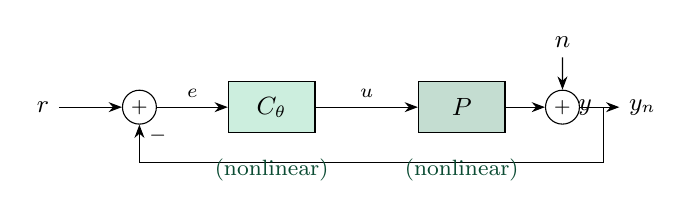
\begin{tikzpicture}[>=Stealth, node distance=1.0cm, font=\small,box/.style={draw, rectangle, minimum width=1.1cm, minimum height=0.65cm}]
        \node[box, fill=midgreen!25] (P) {$P$};
        \node[box, fill=accentgreen!20, left=1.3cm of P] (C) {$C_\theta$};
        \node[circle, draw, inner sep=1.5pt, left=0.9cm of C] (sum) {\scriptsize$+$};
        \node[left=0.8cm of sum] (r) {$r$};
        \node[right=0.8cm of P] (y) {$y$};
        \node[above right=0.3cm and 0.5cm of P] (n) {$n$};
        \node[circle, draw, inner sep=1.5pt, right=0.5cm of P] (nadd) {\scriptsize$+$};
        \node[right=0.5cm of nadd] (yn) {$y_n$};
        \draw[->] (r) -- (sum);
        \draw[->] (sum) -- node[above]{\scriptsize$e$} (C);
        \draw[->] (C) -- node[above]{\scriptsize$u$} (P);
        \draw[->] (P) -- (nadd);
        \draw[->] (n) -- (nadd);
        \draw[->] (nadd) -- (yn);
        \draw[->] ($(nadd.east)+(0.3,0)$) -- ++(0,-0.7) -| ($(sum.south)$) node[pos=0.85,right]{\scriptsize$-$};
        \node[below=0.2cm of C, font=\footnotesize, text=darkgreen] {(nonlinear)};
        \node[below=0.2cm of P, font=\footnotesize, text=darkgreen] {(nonlinear)};
      \end{tikzpicture}
      \vspace{0.3em}
      \begin{exampleblock}{Key Assumptions}
        \begin{itemize}\small
          \item \textbf{A.1}: $p$ is smooth
          \item \textbf{A.2}: $P$ is \emph{invertible} (as a map $u \to y$)
          \item \textbf{A.3}: $c$ is smooth in $\theta$
          \item \textbf{A.4}: Reference model $M$ is lower-triangular \& invertible
        \end{itemize}
      \end{exampleblock}
    \end{column}
  \end{columns}
\end{frame}

% ─────────────────────────────────────────────────────────────────────────────
\begin{frame}{Control Objective \& Reference Model}
  \begin{columns}[T]
    \begin{column}{0.50\textwidth}
      \begin{block}{Reference Model $M$}
        A linear causal invertible map $r \to y$:
        \[
          M(z^{-1}) = \frac{b_1 z^{-1}+\cdots+b_{n_{M_r}}z^{-n_{M_r}}}{1 + a_1 z^{-1}+\cdots+a_{n_{M_y}}z^{-n_{M_y}}}
        \]
        in the time domain:
        \small
        \[
          y(t) = -a_1 y(t-1) - \cdots + b_1 r(t-1) + \cdots + b_{n_{M_r}} r(t-n_{M_r})
        \]
        \normalsize
        \textbf{Why linear $M$?} Bandwidth, frequency response, and intuitive tuning knobs still apply.
      \end{block}
    \end{column}
    \begin{column}{0.47\textwidth}
      \begin{block}{Formal Control Objective}
        \[
          \min_\theta \; \Jopt(\theta) := \bigl\|y_\theta - M[\tilde{r}]\bigr\|^2
        \]
        where $y_\theta = P[C_\theta[\tilde{r} - Dy_\theta]]$ is the closed-loop output and $D$ is the delay matrix.
      \end{block}
      \vspace{0.3em}
      \begin{alertblock}{The Core Problem}
        $\Jopt(\theta)$ \textbf{depends on the unknown plant $P$} and cannot be minimized directly.\\[0.4em]
        VRFT replaces $\Jopt(\theta)$ with a \highlight{data-computable surrogate} $\JJ(\theta)$.
      \end{alertblock}
    \end{column}
  \end{columns}
\end{frame}

% ══════════════════════════════════════════════════════════════════════════════
\section{The VRFT Approach}
% ══════════════════════════════════════════════════════════════════════════════

\begin{frame}{The Virtual Reference Idea}
  \begin{columns}[T]
    \begin{column}{0.50\textwidth}
      \begin{block}{Key Insight}
        Given collected output $\tilde{y}$, define the \emph{virtual reference}:
        \[
          \tilde{r} := M^{-1}[\tilde{y}]
        \]
        \begin{itemize}
          \item $\tilde{r}$ is ``virtual'' --- it was \emph{not} the actual reference during data collection
          \item It only exists in the computer, computed from data
          \item Interpretation: $\tilde{r}$ is the reference for which we would be \emph{happy} to see $\tilde{y}$ as the output (since $M[\tilde{r}] = \tilde{y}$)
        \end{itemize}
      \end{block}
    \end{column}
    \begin{column}{0.47\textwidth}
      \begin{exampleblock}{Virtual Error}
        \[
          \tilde{e} = \tilde{r} - D\tilde{y}
        \]
        A good controller should satisfy:
        \[ C_\theta[\tilde{e}] = \tilde{u} \]
        because: $P[\tilde{u}]$ generates $\tilde{y}$ (measured), and the desired output when reference is $\tilde{r}$ is also $\tilde{y}$.
      \end{exampleblock}
      \vspace{0.3em}
      \begin{block}{VRFT Surrogate Cost}
        \[
          \JJ(\theta) := \bigl\|F[C_\theta[\tilde{e}]] - F[\tilde{u}]\bigr\|^2
        \]
        \highlight{No $P$ appears} --- fully data-computable!
      \end{block}
    \end{column}
  \end{columns}
\end{frame}

% ─────────────────────────────────────────────────────────────────────────────
\begin{frame}{Theorem 1: Perfect Matching Case}
  \begin{columns}[T]
    \begin{column}{0.55\textwidth}
      \begin{block}{Theorem 1 (Perfect Matching)}
        If $\theta_0$ gives perfect tracking, i.e.\
        \[
          \|y_{\theta_0} - M[\tilde{r}]\|^2 = 0,
        \]
        then $\theta_0$ is a minimizer of $\JJ(\theta) = \|F[C_\theta[\tilde{e}]] - F[\tilde{u}]\|^2$.
      \end{block}
      \vspace{0.4em}
      \begin{block}{Proof Sketch}
        Perfect tracking: $y_{\theta_0} = \tilde{y}$.\\
        Since $P[\tilde{u}] = \tilde{y}$ and $P[C_{\theta_0}[\tilde{r}-Dy_{\theta_0}]] = \tilde{y}$,\\
        invertibility of $P$ (A.2) gives $C_{\theta_0}[\tilde{e}] = \tilde{u}$,\\
        hence $\JJ(\theta_0) = 0$, and $\JJ \geq 0$. \qquad $\square$
      \end{block}
    \end{column}
    \begin{column}{0.42\textwidth}
      \begin{exampleblock}{Key Consequence}
        \begin{itemize}
          \item We set out to minimize $\Jopt(\theta)$ --- a \emph{non-convex, $P$-dependent} function
          \item $\JJ(\theta)$ is different from $\Jopt(\theta)$
          \item Yet they share the \highlight{same global minimizer} when perfect matching is possible
          \item For \emph{linearly parameterized} controllers: $\JJ(\theta)$ is \highlight{quadratic} $\Rightarrow$ easy to minimize!
        \end{itemize}
      \end{exampleblock}
      \vspace{0.3em}
      \textbf{What if perfect matching fails?} $\Rightarrow$ Role of filter $F$.
    \end{column}
  \end{columns}
\end{frame}

% ─────────────────────────────────────────────────────────────────────────────
\begin{frame}{Worked Example: Theorem 1 Illustration}
  \begin{columns}[T]
    \begin{column}{0.46\textwidth}
      \begin{exampleblock}{Setup}
        Plant: $y(t) = y(t-1) + u(t-1)^3$\\
        Controller class: $u(t) = \theta\, e(t)^{1/3}$\\
        Reference model: $M = I$ \; $\Rightarrow$ $y(t) = r(t-1)$\\[0.4em]
        Run for $N=2$ with $\tilde{u}(0)=\tilde{u}(1)=1$:\\
        $\tilde{y}(1)=1$, $\tilde{y}(2)=2$, $\tilde{r}(0)=1$, $\tilde{r}(1)=2$
      \end{exampleblock}
      \vspace{0.3em}
      \begin{block}{True Cost (requires knowing $P$)}
        \[
          \Jopt(\theta) = (\theta^3-1)^2 + (3\theta^3-\theta^6-2)^2
        \]
        Minimized at $\theta_0 = 1$ (perfect tracking).
      \end{block}
    \end{column}
    \begin{column}{0.51\textwidth}
      \begin{block}{VRFT Cost ($F=I$, no plant needed)}
        $\tilde{e}(0)=\tilde{r}(0)-\tilde{y}(0)=1$, $\tilde{e}(1)=\tilde{r}(1)-\tilde{y}(1)=1$
        \[
          \JJ(\theta) = (\theta \cdot 1^{1/3}-1)^2 + (\theta \cdot 1^{1/3}-1)^2 = 2-4\theta+2\theta^2
        \]
        Minimized at $\theta_0 = 1$. \highlight{Same minimizer!}
      \end{block}
      \vspace{0.3em}
      \begin{alertblock}{Important Feature}
        While $\Jopt(\theta)$ is a complex degree-12 polynomial (generally highly non-convex), $\JJ(\theta)$ is \highlight{quadratic} for linearly parameterized controllers. Both are minimized at the same $\theta_0$.
      \end{alertblock}
    \end{column}
  \end{columns}
\end{frame}

% ══════════════════════════════════════════════════════════════════════════════
\section{Filter Design}
% ══════════════════════════════════════════════════════════════════════════════

\begin{frame}{Why a Pre-Filter $F$ Is Needed}
  \begin{columns}[T]
    \begin{column}{0.50\textwidth}
      \begin{alertblock}{When Perfect Matching Fails}
        In practice, the controller class $\{C_\theta\}$ is \emph{restricted} (e.g., PI/PID). The ideal controller $C^0 = P^{-1}(I-MD)^{-1}M$ may not belong to the class.\\[0.4em]
        In this case, $\Jopt$ and $\JJ$ (without filter) share the same global minimizer \emph{over the full space} but \textbf{not} when restricted to the controller class.
      \end{alertblock}
      \vspace{0.3em}
      \begin{block}{Filter Goal}
        Choose $F$ such that the second-order derivatives of $\JJ$ and $\Jopt$ \textbf{match at the minimizer}:
        \[
          \frac{\partial^2 \JJ(\theta^+)}{\partial{\theta^+}^2}\Bigg|_{\theta^+_0}
          = \frac{\partial^2 \Jopt(\theta^+)}{\partial{\theta^+}^2}\Bigg|_{\theta^+_0}
        \]
      \end{block}
    \end{column}
    \begin{column}{0.47\textwidth}
      \begin{block}{The Ideal Controller}
        Define $C^0 := P^{-1}(I-MD)^{-1}M$\\[0.3em]
        If placed in the loop: closed-loop $r \to y$ is exactly $M$.\\[0.3em]
        Used for \emph{analysis only} --- never computed in practice.
      \end{block}
      \vspace{0.3em}
      \begin{exampleblock}{Extended Class Trick}
        Expand the controller class:
        \[ \theta^+ = [\theta^T\;\tilde\theta]^T, \quad C_{\theta^+} = C_\theta + \tilde\theta(C^0 - C_0) \]
        \begin{itemize}
          \item $C^0$ obtained at $\theta^+_0 = [0^T\;1]^T$
          \item Original class: $\tilde\theta = 0$
          \item Matching second derivatives in extended class ensures near-optimality in original class
        \end{itemize}
      \end{exampleblock}
    \end{column}
  \end{columns}
\end{frame}

% ─────────────────────────────────────────────────────────────────────────────
\begin{frame}{Theorem 2: The Optimal Filter}
  \begin{columns}[T]
    \begin{column}{0.53\textwidth}
      \begin{block}{Theorem 2 (Filter Design)}
        If the pre-filter is chosen as:
        \[
          \boxed{F = (I - MD)\left(\frac{\partial P[u]}{\partial u}\bigg|_{\tilde{u}}\right)}
        \]
        then the second-order derivatives of $\JJ(\theta^+)$ and $\Jopt(\theta^+)$ match at $\theta^+_0$ (the extended ideal point).
      \end{block}
      \vspace{0.4em}
      \begin{block}{Two Components of $F$}
        \begin{enumerate}
          \item $\displaystyle\frac{\partial P[u]}{\partial u}\Big|_{\tilde{u}}$: incremental linearization of $P$ around $\tilde{u}$ --- accounts for input-to-output effect
          \item $(I - MD)$: de-emphasizes frequencies where $M \approx 1$ (i.e., where tracking is already easy)
        \end{enumerate}
      \end{block}
    \end{column}
    \begin{column}{0.44\textwidth}
      \begin{exampleblock}{Interpretation of $F$}
        \begin{itemize}
          \item The closed-loop cost $J$ is less sensitive to errors where $M \approx 1$
          \item $\JJ$ (open-loop cost) does not incorporate this automatically
          \item Filter $F$ \highlight{artificially injects} the closed-loop sensitivity weighting into the open-loop cost
          \item Net effect: $F$ acts like a \textbf{high-pass filter} --- emphasizes transient, attenuates steady-state
        \end{itemize}
      \end{exampleblock}
      \vspace{0.2em}
      \begin{alertblock}{Estimating $\partial P / \partial u$}
        The Jacobian $\partial P[u]/\partial u|_{\tilde{u}}$ must be estimated from data (e.g., via forgetting-factor identification). Imprecision here only affects second derivatives, not optimality in the perfect-matching case.
      \end{alertblock}
    \end{column}
  \end{columns}
\end{frame}

% ─────────────────────────────────────────────────────────────────────────────
\begin{frame}{Filter: Linear Case Comparison}
  \begin{columns}[T]
    \begin{column}{0.48\textwidth}
      \begin{block}{Linear VRFT Filter (Campi et al.\ 2002)}
        \[
          F_{\mathrm{lin}} = (1-M)\,M\,\frac{1}{\Phi_u^{1/2}}
        \]
        (stationary, frequency domain)\\[0.4em]
        Matched model-reference complementary sensitivity cost, for \emph{any} reference signal.
      \end{block}
    \end{column}
    \begin{column}{0.48\textwidth}
      \begin{block}{Nonlinear VRFT Filter (this paper)}
        \[
          F_{\mathrm{nl}} = (I-MD)\left(\frac{\partial P[u]}{\partial u}\bigg|_{\tilde{u}}\right)
        \]
        (time-variant operator)\\[0.4em]
        Matches cost for the \emph{specific} reference $\tilde{r} = M^{-1}[\tilde{y}]$.
      \end{block}
    \end{column}
  \end{columns}
  \vspace{0.5em}
  \begin{exampleblock}{Connecting the Two}
    In linear stationary notation: $(I-MD)\,(\partial P/\partial u)|_{\tilde{u}} \;\to\; (1-M)\,P\,\Phi_{\tilde{u}}^{1/2}$.\\
    Adding the specific-reference term $M^{-1}P\Phi_{\tilde{u}}^{1/2}$ recovers the linear filter exactly, confirming the nonlinear filter as the correct generalization.
  \end{exampleblock}
\end{frame}

% ─────────────────────────────────────────────────────────────────────────────
\begin{frame}{Example: Under-Parameterized PI Controller}
  \begin{columns}[T]
    \begin{column}{0.40\textwidth}
      \begin{exampleblock}{Setup}
        \small
        Plant: $y(t) = 0.9y(t-1) + \tanh(u(t-1))$\\
        Reference model: $y(t) = r(t-1)$ ($M = I$)\\[0.3em]
        \textbf{Ideal controller:}
        $u(t) = \tanh^{-1}(v(t))$ (complex nonlinear system)\\[0.3em]
        \textbf{Controller class:} PI
        \[
          u(t) = \left(\frac{0.2}{1-z^{-1}} + \theta\right)e(t)
        \]
        (integral fixed; proportional $\theta$ selected by VRFT)
      \end{exampleblock}
    \end{column}
    \begin{column}{0.57\textwidth}
      \begin{block}{Observations from Contour Plots}
        \begin{itemize}
          \item \textbf{All three 2D indices} ($J(\theta^+)$, $\JJ$ filtered, $\JJ$ unfiltered) share the same full-space minimum (confirming Theorem 1 for perfect matching case)
          \item \textbf{$\JJ$ (unfiltered)} is quadratic but its shape differs drastically from $J(\theta^+)$; PI slice minimizer drifts far from $J$'s minimizer
          \item \textbf{$\JJ$ (filtered)} is rotated/warped to match the 2nd-order expansion of $J$ around the minimum; PI slice minimizer closely tracks $J$'s minimizer
          \item Filter effect on $\tilde{u}$: \highlight{high-pass} --- transient emphasized, steady-state attenuated
        \end{itemize}
      \end{block}
    \end{column}
  \end{columns}
\end{frame}

% ══════════════════════════════════════════════════════════════════════════════
\section{Implementation}
% ══════════════════════════════════════════════════════════════════════════════

\begin{frame}{Implementation: Quadratic Optimization}
  \begin{columns}[T]
    \begin{column}{0.50\textwidth}
      \begin{block}{Linearly Parameterized Controllers}
        If $C_\theta[\tilde{e}] = \theta_1 s_1(\tilde{e}) + \cdots + \theta_{n_\theta} s_{n_\theta}(\tilde{e})$
        (where $s_i$ may be nonlinear), then:
        \[
          F[C_\theta[\tilde{e}]] = F[C[\tilde{e}]]\,\theta
        \]
        and $\JJ(\theta)$ is \highlight{quadratic}:
        \[
          \JJ(\theta) = \|F[C[\tilde{e}]]\,\theta - F[\tilde{u}]\|^2
        \]
      \end{block}
      \vspace{0.3em}
      \begin{block}{Closed-Form Solution}
        \[
          \hat\theta = \bigl(F[C[\tilde{e}]]^T F[C[\tilde{e}]]\bigr)^{-1} F[C[\tilde{e}]]^T F[\tilde{u}]
        \]
        i.e., solve the normal equations:
        \[
          F[C[\tilde{e}]]^T\bigl(F[C[\tilde{e}]]\,\hat\theta - F[\tilde{u}]\bigr) = 0
        \]
      \end{block}
    \end{column}
    \begin{column}{0.47\textwidth}
      \begin{exampleblock}{Algorithm Summary (Noise-Free)}
        \begin{enumerate}
          \setlength{\itemsep}{0.4em}
          \item \textbf{Data collection:} obtain $\{\tilde{u}, \tilde{y}\}$
          \item \textbf{Virtual reference:} $\tilde{r} = M^{-1}[\tilde{y}]$
          \item \textbf{Virtual error:} $\tilde{e} = \tilde{r} - D\tilde{y}$
          \item \textbf{Estimate Jacobian:} identify $\partial P[u]/\partial u|_{\tilde{u}}$ (e.g., forgetting-factor method)
          \item \textbf{Form filter:} $F = (I-MD)\cdot(\partial P/\partial u)|_{\tilde{u}}$
          \item \textbf{Apply filter:} compute $F[C[\tilde{e}]]$ and $F[\tilde{u}]$
          \item \textbf{Solve least squares:} obtain $\hat\theta$ in closed form
        \end{enumerate}
      \end{exampleblock}
    \end{column}
  \end{columns}
\end{frame}

% ─────────────────────────────────────────────────────────────────────────────
\begin{frame}{Handling Noisy Data}
  \begin{columns}[T]
    \begin{column}{0.50\textwidth}
      \begin{alertblock}{Noisy Measurement Model}
        \[
          \tilde{y}_n(t) = \tilde{y}(t) + \tilde{n}(t)
        \]
        Leads to a \emph{noisy regressor matrix}:
        \[
          F[C[\tilde{e}_n]] = F[C[\tilde{e}]] + \Psi
        \]
        where $\Psi$ is the noise component.\\[0.4em]
        Standard LS gives a \alerttext{biased} estimate $\hat\theta_n \neq \hat\theta$ when $\Psi \neq 0$.
      \end{alertblock}
    \end{column}
    \begin{column}{0.47\textwidth}
      \begin{exampleblock}{Instrumental Variable (IV) Fix}
        Run a \emph{second} experiment with same input $\tilde{u}$, collect $\tilde{y}^*_n = \tilde{y} + \tilde{n}^*$.\\[0.3em]
        Since $\tilde{n}$ and $\tilde{n}^*$ are independent:
        \[
          F[C[\tilde{e}^*_n]]^T\bigl(F[C[\tilde{e}_n]]\,\hat\theta^* - F[\tilde{u}]\bigr) = 0
        \]
        $\hat\theta^* \approx \hat\theta$ (consistent as $N\to\infty$)
      \end{exampleblock}
      \vspace{0.3em}
      \begin{block}{Note on Nonlinear Case}
        IV noise handling for \emph{nonlinearly} parameterized controllers is more complex --- identified as an open problem.
      \end{block}
    \end{column}
  \end{columns}
\end{frame}

% ══════════════════════════════════════════════════════════════════════════════
\section{Multipass Refinement}
% ══════════════════════════════════════════════════════════════════════════════

\begin{frame}{Multipass Procedure for Reference Refinement}
  \begin{columns}[T]
    \begin{column}{0.50\textwidth}
      \begin{block}{Motivation}
        In one-shot VRFT, $\tilde{r} = M^{-1}[\tilde{y}]$ may differ from the actual desired reference $\bar{r}$.\\[0.3em]
        This is usually fine (if $\tilde{u}$ is exciting enough, the designed controller works for a broad class of signals).\\[0.3em]
        But when a \emph{specific} $\bar{r}$ matters, a multipass refinement can be used.
      \end{block}
      \vspace{0.4em}
      \begin{block}{Iterative Scheme}
        At pass $k$, controller $C_k$ in loop:
        \begin{enumerate}
          \item Inject $\bar{r}$; measure output $y_k$
          \item Compute $\tilde{r}_{k+1} = M^{-1}[y_k]$
          \item Apply VRFT with $\tilde{r}_{k+1}$ to get $C_{k+1}$
        \end{enumerate}
      \end{block}
    \end{column}
    \begin{column}{0.47\textwidth}
      \begin{exampleblock}{Linear Case: One-Step Convergence}
        If the closed-loop operator $H_k$ is invertible:
        \[
          \delta_{k+1} = H_{k+1}\bar{r} - M\bar{r} = 0
        \]
        i.e., the virtual reference is exactly $\bar{r}$ after \highlight{one} extra pass.\\[0.3em]
        Moreover, $H_{k+1}$ has ``learned'' to compensate for the mismatch $\delta_k$.
      \end{exampleblock}
      \vspace{0.3em}
      \begin{block}{Nonlinear Case: Contraction}
        Under mild assumption (A.4: $\rho$-contraction), $\delta_k \to 0$ as $k \to \infty$.\\[0.3em]
        Connections to \emph{repetitive process} theory; convergence analysis is a direction for further work.
      \end{block}
    \end{column}
  \end{columns}
\end{frame}

% ══════════════════════════════════════════════════════════════════════════════
\section{Summary \& Conclusions}
% ══════════════════════════════════════════════════════════════════════════════

\begin{frame}{Summary of the Nonlinear VRFT Method}
  \begin{columns}[T]
    \begin{column}{0.55\textwidth}
      \begin{exampleblock}{Key Contributions}
        \begin{enumerate}
          \setlength{\itemsep}{0.35em}
          \item \textbf{Extension to nonlinear plants}: first one-shot direct data-based method for nonlinear controller tuning
          \item \textbf{Theorem 1}: VRFT cost shares global minimizer with true control cost when perfect matching is achievable
          \item \textbf{Theorem 2}: optimal pre-filter $F=(I-MD)(\partial P/\partial u)|_{\tilde{u}}$ ensures near-optimality in under-parameterized (restricted) settings
          \item \textbf{Quadratic optimization}: for linearly parameterized controllers, $\JJ(\theta)$ is quadratic $\to$ closed-form solution
          \item \textbf{Noise handling}: IV approach with two experiments
          \item \textbf{Multipass refinement}: iterative scheme targeting a specific reference signal
        \end{enumerate}
      \end{exampleblock}
    \end{column}
    \begin{column}{0.42\textwidth}
      \begin{alertblock}{Limitations \& Open Issues}
        \begin{itemize}
          \item Invertibility of $P$ (A.2) may be restrictive for some nonlinear plants
          \item Filter requires estimating $\partial P/\partial u|_{\tilde{u}}$: adds a semi-indirect step
          \item Stability of designed closed-loop not guaranteed --- must be verified separately
          \item IV noise handling for nonlinearly parameterized controllers: open problem
          \item Convergence analysis for nonlinear multipass: partial results only
        \end{itemize}
      \end{alertblock}
    \end{column}
  \end{columns}
\end{frame}

% ─────────────────────────────────────────────────────────────────────────────
\begin{frame}{Placing Nonlinear VRFT in Context}
  \begin{center}
  \renewcommand{\arraystretch}{1.3}
  \begin{tabular}{lccc}
    \toprule
    \textbf{Method} & \textbf{Nonlinear} & \textbf{One-Shot} & \textbf{Direct} \\
    \midrule
    Ziegler--Nichols (1942) & $\times$ & \checkmark & \checkmark \\
    Linear VRFT (2002) & $\times$ & \checkmark & \checkmark \\
    Nonlinear IFT (1998--2004) & \checkmark & $\times$ (iterative) & \checkmark \\
    \textbf{Nonlinear VRFT (this paper)} & \checkmark & \checkmark & \checkmark \\
    \bottomrule
  \end{tabular}
  \end{center}
  \vspace{0.5em}
  \begin{columns}[T]
    \begin{column}{0.48\textwidth}
      \begin{block}{Notable Applications (at time of publication)}
        \begin{itemize}
          \item MIMO process control (Nakamoto 2004)
          \item Robot motion control (Kostic 2004)
          \item Neuroprostheses / FES control (Previdi et al.\ 2004, 2005)
          \item Non-minimum phase systems (Sala \& Esparza 2005)
        \end{itemize}
      \end{block}
    \end{column}
    \begin{column}{0.48\textwidth}
      \begin{exampleblock}{Relation to Linear VRFT}
        All results reduce cleanly to the 2002 linear VRFT paper when $P$ is linear and stationary. The filter $F$ coincides with $(1-M)M/\Phi_u^{1/2}$, confirming the nonlinear result as a true generalization.
      \end{exampleblock}
    \end{column}
  \end{columns}
\end{frame}

% ─────────────────────────────────────────────────────────────────────────────
\begin{frame}[plain]
  \begin{center}
    \vspace{1.5em}
    {\Large\color{darkgreen}\textbf{Thank You}}\\[1em]
    \rule{0.55\textwidth}{0.5pt}\\[1em]
    \textbf{Reference:}\\[0.4em]
    M.C.~Campi, S.M.~Savaresi\\
    \textit{Direct Nonlinear Control Design: The Virtual Reference Feedback Tuning (VRFT) Approach}\\
    \textbf{IEEE Transactions on Automatic Control}, 51(1):14--27, January 2006\\[1.5em]
    \rule{0.55\textwidth}{0.5pt}\\[0.8em]
    {\small Predecessor:} M.C.~Campi, A.~Lecchini, S.M.~Savaresi\\
    {\small \textit{Virtual Reference Feedback Tuning}, \textbf{Automatica} 38(8), 2002}
  \end{center}
\end{frame}

\end{document}
